\section{Indecidibilità}
\subsection{Metodo della diagonalizzazione}

Tale metodo è un metodo scoperto da Cantor nel 1873, e serve per confrontare le dimensioni di \g{insiemi infiniti}.

\g{due insiemi finiti hanno la stessa dimensione se gli elementi di un insieme possono essere accoppiati agli elementi dell'altro insieme}

\paragraph{Corrispondenze}
Abbiamo due insiemi $A$ e $B$ e una funzione $f:A\rightarrow B$ 
\begin{itemize}
	\item $f$ è \g{iniett} se non mappa mai elementi diversi nello stesso punto: $f(a)\neq f(b)$ ogniqualvolta che $a\neq b$ 
	\item $f$ è \g{suriettiva} se tocca ogni elemento di $B$: 
  	Per ogni $b\in B$ esiste $a\in A$ tale che $f(a)=b$ 
	\item Una funzione iniettiva e suriettiva è chiamata \g{biettiva}: è un modo per \g{accoppiare} elementi di $A$ con elementi di $B$ 
\end{itemize}
\paragraph{Definizione}
$A$ e $B$ hanno la \g{stessa cardinalità} se esiste una funzione \g{biettiva} $f:A\rightarrow B$ 

\subsection{Esempio: naturali vs numeri pari}
\begin{itemize}
	\item $\mathbb{N}=\{0,1,2,\dots\}$, insieme dei numeri naturali.
	\item $\mathbb{E} = \{0,2,4,\dots\}$, insieme dei numeri pari.
\end{itemize}
\g{Quale dei due insiemi è il più grande?}\\

\paragraph{Definizione di insieme numerabile} 
Un insieme è \g{numerabile} se è finito oppure la la stessa cardinalità di $\mathbb{N}$ 

\paragraph{Altri esempi}
\begin{itemize}
	\item $\mathbb{Q}$ è numerabile? 
	\item $\mathbb{R}$ è numerabile? 
	\item Dato un alfabeto finito $\Sigma$, $\Sigma^*$ è numerabile? 
	\item L'insieme di \g{tutte le macchine di Turing} è numerabile? 
	\item L'insieme di \g{tutte le sequenze binarie infinite} è numerabile? 
	\item Dato un alfabeto finito $\Sigma$, l'insieme di \g{tutti i linguaggi} su $\Sigma^*$ è numerabile? 
\end{itemize}

\paragraph{Corollario}
\begin{itemize}
	\item L'insieme di tutte le macchine di Turing è \g{numerabile} 
	\item L'insieme di tutti i linguaggi è \g{non numerabile} 
	\item \g{devono} esistere linguaggi non riconoscibili da una macchina di Turing 
\end{itemize}

\subsection{Un risultato fondamentale}
\textit{Esiste un problema specifico che è algoritmicamente \g{irrisolvibile}}
\begin{itemize}
	\item Problemi di interesse non solo teorico, ma anche pratico.
	\item Esempio: Verifica del software: 
\end{itemize}
Verificare che un programma è corretto non è risolvibile algoritmicamente 
\begin{theorem}
	$A_{TM}$ è indecidibile
\end{theorem}
$A_{TM}=\{\langle M,w\rangle\mid M$ è una TM che accetta la stringa $w\}$ 
\begin{itemize}
	\item \g{Chiarimento}: $A_{TM}$ è Turing-riconoscibile
	\item Conseguenza: i riconoscitori **sono più potenti** dei decisori
	\item $U=$ ``Su input $\langle M,w\rangle$, dove $M$ è una TM e $w$ una stringa: 
		1. Simula $M$ su input $w$ 
		2. Se la simulazione raggiunge lo stato di accettazione, \g{accetta}; se raggiunge lo stato di rifiuto, \textit{rifiuta}.''
	\item $U$ è un \g{riconoscitore}. Perché non è un \g{decisore}? 
\end{itemize}

\subsection{Macchina Universale di Turing}
$U$ è un esempio di \g{Macchina Universale di Turing} 
Introdotta da Alan Turing nel 1936, può simulare \g{qualsiasi macchina di Turing} a partire dalla sua descrizione. 

\begin{theorem}
	$A_{TM}$ è indecidibile
\end{theorem}
$A_{TM}= \{\langle M,w\rangle\mid M$ è una TM che accetta la stringa $W\}$ 
\paragraph{Dimostrazione}
\begin{itemize}
	\item Per contraddizione. Assumiamo $A_{TM}$ decidibile per poi trovare una contraddizione
	\item Supponiamo $H$ decisore per $A_{TM}$ 
	\item Cosa fa $H$ con input $\langle M,w\rangle$ ?
\end{itemize}
$H(\langle M,w\rangle)=$ \g{accetta} se $M$ accetta $w$, \textit{rifiuta} altrimenti
\begin{itemize}
\item Definiamo una TM $D$  che usa $H$ come subroutine 
\item $D=$ ``Su input $\langle M\rangle$, dove $M$ è una TM: 
	\begin{enumerate}
		\item Esegue $H$ su input $\langle M,\langle M\rangle\rangle$
		\item  Dà in output l'opposto dell'output di $H$, se $H$ accetta, \textit{rifiuta}; se $H$ rifiuta, \g{accetta} 
	\end{enumerate}
\item Cosa fa $D$ con input $\langle D\rangle$ ? 
$D(\langle D\rangle)=$ \g{accetta} se $D$ non accetta $\langle D\rangle$, \textit{rifiuta} altrimenti.
\end{itemize}
\g{Questa è una contraddizione!}

\paragraph{Comprendere la dimostrazione}
\begin{enumerate}
	\item H accetta $\langle M,w\rangle$ esattamente quando $M$ accetta $w$ 
		\begin{enumerate}
			\item  Banale: abbiamo assunto che $H$ esista e decida $A_{TM}$ 
			\item $M$ rappresenta **qualsiasi** TM e $w$ è una **qualsiasi** stringa 
		\end{enumerate}
	\item $D$ rifiuta $\langle M\rangle$ esattamente quando $M$ acetta $\langle M \rangle$ 
		\begin{enumerate}
			\item Cosa è successo a $w$? 
			\item $w$ è solo una stringa, come $\langle M \rangle$. Tutto ciò che stiamo facendo è definire quale stringa dare in input alla macchina. 
		\end{enumerate}
	\item $D$ rifiuta $\langle D\rangle$ esattamente quando $D$ accetta $\langle D\rangle$ \\
		 Questa è la contraddizione 
	\item Dove si usa la diagonalizzazione? 
\end{enumerate}

\subsection{Un linguaggio non Turing-riconoscibile}
\begin{itemize}
	\item Abbiamo visto che $A_{TM}$ è \g{Turing-riconoscibile} 
	\item Sappiamo che l'insieme di \g{tutte le TM} è \g{numerabile} 
	\item Sappiamo che l'insieme di \g{tutti i linguaggi} è \g{non numerabile} 
	\item Di conseguenza \g{deve} esistere un linguaggio non \g{Turing-riconoscibile} 
\end{itemize}

C'è ancora una cosa che dobbiamo fare prima di poter mostrare un linguaggio non \g{Turing-riconoscibile}.\\
Mostreremo che se un linguaggio e il suo complementare sono Turing-riconoscibili, allora il linguaggio è decidibile. \\
Un linguaggio è \g{co-Turing riconoscibile} se è il complementare di un linguaggio Turing-riconoscibile
\begin{theorem}
	Un linguaggio è decidibile se e solo se è Turing-riconoscibile e co-Turing riconoscibile.
\end{theorem}
\paragraph{Dimostrazione}
\begin{itemize}
	\item Dobbiamo dimostrare entrambe le direzioni 
	\item Se $A$ è decidibile, allora sia $A$ che $\overline{A}$ sono Turing-riconoscibili
		\begin{itemize}
			\item Il complementare di un linguaggio decidibile è decidibile! \end{itemize}
	\item Se $A$ e $\overline{A}$ sono Turing-riconoscibili, possiamo costruire un decisore per $A$ 
\end{itemize}

\subsection{$\overline{A_{TM}}$ non è Turing-riconoscibile}
Se il complementare di $A_{TM}$ fosse Turing-riconoscibile, allora $A_{TM}$ sarebbe decidibile.
Sappiamo che $A_{TM}$ non è decidibile, quindi il suo complementare non può essere Turing-riconoscibile! 
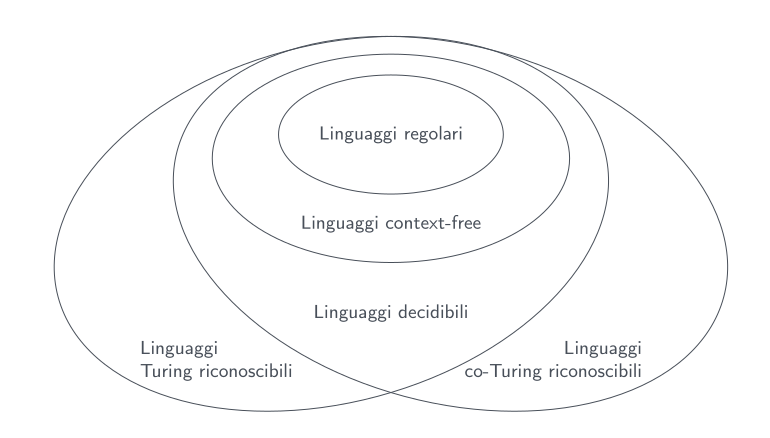
\includegraphics[scale=0.5]{img/linguaggi_diagramma.png}
